\documentclass{article}
\usepackage[utf8]{inputenc}
\usepackage[T1]{fontenc}
\usepackage{textcomp}
\usepackage{amsmath,amssymb}
\usepackage{lmodern}
\usepackage[a4paper]{geometry}
\usepackage{graphicx}
\usepackage{xcolor}
\usepackage{microtype}
\usepackage{hyperref}
\usepackage{diagbox}
\usepackage{booktabs}
\usepackage{listings}
\usepackage[francais]{babel}
\definecolor{darkWhite}{rgb}{0.94,0.94,0.94}
\lstset{
  aboveskip=3mm,
  belowskip=-2mm,
  backgroundcolor=\color{darkWhite},
  basicstyle=\footnotesize,
  breakatwhitespace=false,
  breaklines=true,
  captionpos=b,
  commentstyle=\color{red},
  deletekeywords={...},
  escapeinside={\%*}{*)},
  extendedchars=true,
  framexleftmargin=16pt,
  framextopmargin=3pt,
  framexbottommargin=6pt,
  frame=tb,
  keepspaces=true,
  keywordstyle=\color{blue},
  language=C, JavaScript
  literate=
  {²}{{\textsuperscript{2}}}1
  {⁴}{{\textsuperscript{4}}}1
  {⁶}{{\textsuperscript{6}}}1
  {⁸}{{\textsuperscript{8}}}1
  {€}{{\euro{}}}1
  {é}{{\'e}}1
  {è}{{\`{e}}}1
  {ê}{{\^{e}}}1
  {ë}{{\¨{e}}}1
  {É}{{\'{E}}}1
  {Ê}{{\^{E}}}1
  {û}{{\^{u}}}1
  {ù}{{\`{u}}}1
  {â}{{\^{a}}}1
  {à}{{\`{a}}}1
  {á}{{\'{a}}}1
  {ã}{{\~{a}}}1
  {Á}{{\'{A}}}1
  {Â}{{\^{A}}}1
  {Ã}{{\~{A}}}1
  {ç}{{\c{c}}}1
  {Ç}{{\c{C}}}1
  {õ}{{\~{o}}}1
  {ó}{{\'{o}}}1
  {ô}{{\^{o}}}1
  {Õ}{{\~{O}}}1
  {Ó}{{\'{O}}}1
  {Ô}{{\^{O}}}1
  {î}{{\^{i}}}1
  {Î}{{\^{I}}}1
  {í}{{\'{i}}}1
  {Í}{{\~{Í}}}1,
  morekeywords={*,...},
  numbers=left,
  numbersep=10pt,
  numberstyle=\tiny\color{black},
  rulecolor=\color{black},Usine logicielle javascript
  showspaces=false,
  showstringspaces=false,
  showtabs=false,
  stepnumber=1,
  stringstyle=\color{gray},
  tabsize=4,
  title=\lstname,
}
\hypersetup{pdfstartview=XYZ}
\title{TD1 Théorie des graphes}
\author{}
\date{}
\begin{document}
\maketitle{}
$G=(V,E)$ \\
$\mid V \mid =n$ (sommets) \\
$\mid E \mid =m$ (arêtes)
\section*{Exercice 1}
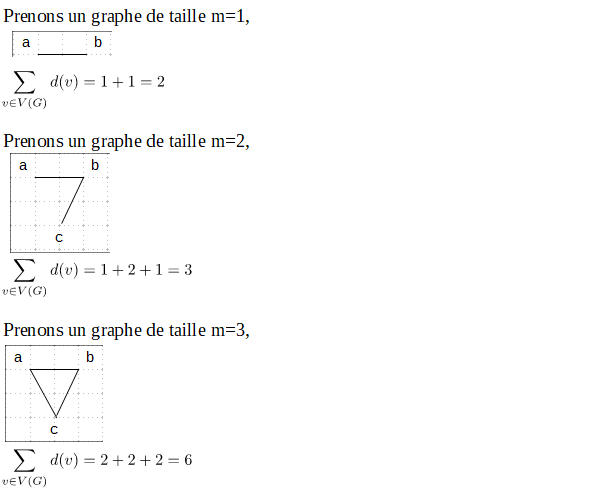
\includegraphics{Image/S1.PNG}
\newpage
Comme chaque arrête u,v va être une fois par u et une fois par v on a toutes les arêtes comptées exactement deux fois. \\
$\sum_{v \in V(G)} d(v)=2m$
\section*{Exercice 2}
Remarque : La somme des degrés est paire (Exercice 1). \\
$\sum_{v \in V(G)} d(v)= \sum_{w \in I(G)} d(w)+\sum_{z \in P(G)} d(z)$ \\
$I(G)=\{v \mid d(v)$ est impair et  $v \in V(G)\}$ \\
$P(G)=\{v \mid d(v) $est pair et$ v \in V(G)\}$ \\
\\
$V=I(G)+P(G)$
\\
Pair + impair -> impair \\
\\
Comme $\sum_{v \in V(G)} d(v)= \sum_{w \in I(G)} d(w)+\sum_{z \in P(G)} d(z)$ -> pair \\
Pour que $\sum_{w \in I(G)} d(w)$ soit pair on a un nombre de sommets de degré impair. 
\section*{Exercice 3}
Un sommet peut avoir max une arrête pour un couple de sommets. \\
On a donc $m_{max}=1+2+3+...+(n-1)={{n^{2}-n} \over 2}$ \\
Les graphes complets atteignent cette borne. \\
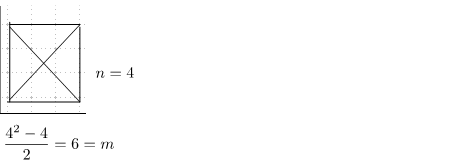
\includegraphics{Image/S2.PNG}
\newpage
\section*{Exercice 4}♦
$\mid E \mid = n-1$ \\
\textbf{Preuve 1 :}  \\
Par récurrence, on va affecter à chaque sommet un numéro unique entre 1 et n. 
Le sous graphes induit par l’ensemble $\{1,…,k\}$ reste un arbre $\forall k \in \{1,…,n\}$. \\
Un arbre est connexe et sans cycle. \\
\begin{center}
Proposition : Dans un arbre il existe un unique chemin entre toute paire de sommets. 
\end{center}
Le graphe $T_i=T(\{1,2,3,…,i\}, E \cap v(T_i))$ \\
$T_1=1 \mid E(T₁) \mid=0$ \\
$T_2=2 \mid E(T_2)\mid=1$ \\
Si c’est vrai par  alors c’est vrai pour $T_{i+1}$ \\
Par hypothèse on a $\mid E(T_i) \mid=i-1$ \\
On ajoute le sommet $i+1$ \\
$i+1$ a exactement un voisin dans $T_{i}$ \\
\\
quand on ajoute le sommet $i+1$ : \\
$\mid V(T_{i+1}) \mid =\mid V(T_i) \mid +1=i+1$\\
$\mid E(T_{i+1}) \mid = \mid E(T_i) \mid +1=i$\\
\\
\textbf{Preuve 2 :} \\
Par bijection, on choisit un sommet arbitrairement et on le désigne racine $r$.
Pour tous les autres sommets différent on oriente les arêtes vers la racine.\\
\\
Pour un sommet particulier $v$ de $T$ différent de $r$, il y a un seul arc incident à $v$ qui soit de $v$ car il existe un unique chemin de $v$ vers $r$ dans $T$. \\
\\
Pour chaque sommet on associe de manière unique le sommet v a son arc sortant $f({v(T) \setminus \{r\}) \rightarrow E$ \\
Tous les sommets ont une unique image sauf $r$. \\
\\
\newpage
\section*{Exercice 5}♣
\section*{Exercice 6}♠
\section*{Exercice 7} 
Soient : \\
(1) T est un arbre \\
(2) Entre toute paire de sommet il existe un unique chemin \\
(3) T est minimale connexe \\♥
(4) T est maximale à cycle \\ 
\\
\subsection*{$(1) \Rightarrow (2)$:}  \\
%Puisque un arbre n'a pas de cycle il y a forcément un unique chemin entre x et y.
Par contraposé, \\
$(1) \Rightarrow (2) \equiv$ $\neg(2) \Rightarrow \neg(1) \\ \exists x,y $ : \\
a) Soit il y a plusieurs chemin entre x et y. $\exists p_1$ et $p_2$ deux chemins distincts entre x et y \\
b) Soit il n'y a pas de chemin entre x et y, donc pas connexe.\\
Il existe un unique chemin $\equiv$ il existe un chemin et il en existe un seul. \\
S'il y a 2 chemin distincts en partant de x, on note z le dernier sommets commun au début de $P_1$ et de $P_2$.\\
On note t le premier sommet qui sont à nouveau commun à $P_1$ et $P_2$. \\
On obtient un cycle de $P_1$ à $P_2$.
\subsection*{$(2) \Rightarrow (3):$}
Par contraposé, \\
$(2) \Rightarrow (3) \equiv$ $\neg(3) \Rightarrow \neg(2) \\ 
\exists e=\{x,y\} $ tq $T \setminus e$ reste connexe. \\
Si $T \setminus e$ est connexe alors il existe un chemin P dans $T \setminus $ qui relie x à y P et e dans T sont deux chemins différents qui relient x à y.
\subsection*{$(3) \Rightarrow (4)$:}
Minimalement connexe : \\
- Connexe et pas de cycle. \\
Si on ajoute une arête entre n'importe quelle pair de sommet, on créé un cycle. \\  
\subsection*{$(4) \Rightarrow (1)$:}
Maximalement acyclique -> acyclique. \\
$\foall x,y$ tel que $x,y \in E(T)$ \\
$E(T)=E(T) \cup \{x,y\}$ \\
On a un cycle dans T il existait déjà un chemin entre x et y.
\newpage
\section*{Exercice 8}
\section*{Exercice 9}
\subsection*{(1)}
Taille en mémoire \\
Matrice d'adjacence : o($n^2$) \\
Matrice d'incidence : o($n \times m$)\\
Liste d'adjacence : o(n+m)\\
\subsection*{(2)}
Temps \\
Matrice d'adjacence :o(1) \\
Matrice d'incidence :o(m) \\
Liste d'adjacence : o($min\{d(x),d(y)\}$)\\
\section*{Exercice 10}
\subsection*{(1) $ \mid E \mid \leq \mid x \mid \times \mid y \mid$}
Les arêtes autorisées ont exactement une extrémité dans X et une autre dans y. \\
$x=\{x_1,x_2,...,x_l\}$ \\
$y=\{y_1,y_2,...y_k\}$ \\
\\
$ l \times k$ couples différents possibles. \\
$l=\mid x \mid$ \\
$k=\mid y \mid$ \\
\subsection*{(2)$\sum_{x \in X} d(x)= \sum_{y \in Y} d(y)$}
$\sum_{x \in X} d(x)= \sum_{y \in Y} d(y)$ \\
Chaque arrête a exactement une extrémité dans X et l'autre dans Y. \\
\subsection*{(3)$\mid E \mid \leq \frac{n^2}{4}$}
$ \mid E \mid \leq \mid x \mid \times \mid y \mid$ \\
On a $ \mid x \mid=\frac{n]{2} $ et $\mid y \mid = \frac(n}{2}$ \\
$\sum d(x)= \frac{n}{2} \times \frac{n}{2}=\frac{n^2}{4}$ \\
\begin{center}
Dans un graphe bipartie quelconque  :
\end{center}
$\mid X \mid=\frac{n}{2}+k$ et $\mid Y \mid=\frac{n}{2}-k$ \newpage
$\frac{n^2}{4}+\frac{kn}{2}+k^2-\frac{kn}{2}-k^2=\frac{n^2}{4}-k^2$ \\
$\forall k \geq 1$ \\☺
On a $n^2 > (\frac{n^2}{4}-k^2)$

\section*{Exercice 11}
\subsection*{0-régulier}
Stable.
\subsection*{1-régulier}
Un ensemble d'arêtes disjointe, nombre de sommet pair.
\subsection*{2-régulier}
Collections de cycle disjointe.
 
\section*{Exercice 12}
\subsection*{(1) non orienté, simple, $\delta(G) > \frac{n-2}{2}$ et connexe}
Par l'absurde, \\
$\delta(G)> \frac{n-2}{2}$ et G n'est pas connexe. \\ 
Si G n'est pas connexe il a au moins deux composantes connexes. \\
On considère ces deux composantes $C_1$ et $C_2$. \\
$\mid C_1 \mid \geq \frac{n}{2}+1 $ \\
$\mid C_2 \mid \geq \frac{n}{2}+1 $ \\
$\mid C_1 + C_2 \mid \geq 2(\frac{n}{2}+1)=n+2$ \\
$\mid C_1 + C_2 \mid \leq n$ \\

Il existe un sommet qui appartient à $C_1$ et $C_2$ donc G est connexe.
\subsection*{(2) n pair, graphe $\frac{n-2}{2}$-régulier simple et pas connexe}
$\frac{n-2}{2} \equiv \frac{n}{2}-1$-régulier \\
Si on prend de 2 clique r-1 régulier \\
2r sommet n=2r \\
$r=\frac{n}{2}$
\newpage
\section*{Exercice 13}
\subsection*{(1) Graphe simple, non orienté, déconnecté $\Longrightarrow$ complémentaire connexe}
G est connexe si et seulement si $\forall_{x,y} \in V(G)$, il existe un chemin de x vers y. \\
Si G pas connexe alors $\overline{G}$ connexe. \\
1-$x \in c_i$, $y \in c_j$ \\
$i \neq j$ \\
une arête va les relier dans $\overline{G}$. \\
\\
2- Pour chaque $C_i$ de $G$ pour toute paire de sommets $x,z \in C_i$ il existe un chemin de $x$ à $z$ dans $\overline{G}$ en utilisant un sommet $y$ de $C_j$ on sait que dans $\overline{G}$ il existe un chemin $x.y$ car y voit tout les sommets de $C_i$.
\subsection*{(2) La réciproque}
Graphe en ligne droite, 4 sommets.
\section*{Exercice 14}
Graphe en largeur.
	

\end{document}
